
%% bare_conf.tex
%% V1.3
%% 2007/01/11
%% by Michael Shell
%% See:
%% http://www.michaelshell.org/
%% for current contact information.
%%
%% This is a skeleton file demonstrating the use of IEEEtran.cls
%% (requires IEEEtran.cls version 1.7 or later) with an IEEE conference paper.
%%
%% Support sites:
%% http://www.michaelshell.org/tex/ieeetran/
%% http://www.ctan.org/tex-archive/macros/latex/contrib/IEEEtran/
%% and
%% http://www.ieee.org/

%%*************************************************************************
%% Legal Notice:
%% This code is offered as-is without any warranty either expressed or
%% implied; without even the implied warranty of MERCHANTABILITY or
%% FITNESS FOR A PARTICULAR PURPOSE! 
%% User assumes all risk.
%% In no event shall IEEE or any contributor to this code be liable for
%% any damages or losses, including, but not limited to, incidental,
%% consequential, or any other damages, resulting from the use or misuse
%% of any information contained here.
%%
%% All comments are the opinions of their respective authors and are not
%% necessarily endorsed by the IEEE.
%%
%% This work is distributed under the LaTeX Project Public License (LPPL)
%% ( http://www.latex-project.org/ ) version 1.3, and may be freely used,
%% distributed and modified. A copy of the LPPL, version 1.3, is included
%% in the base LaTeX documentation of all distributions of LaTeX released
%% 2003/12/01 or later.
%% Retain all contribution notices and credits.
%% ** Modified files should be clearly indicated as such, including  **
%% ** renaming them and changing author support contact information. **
%%
%% File list of work: IEEEtran.cls, IEEEtran_HOWTO.pdf, bare_adv.tex,
%%                    bare_conf.tex, bare_jrnl.tex, bare_jrnl_compsoc.tex
%%*************************************************************************

% *** Authors should verify (and, if needed, correct) their LaTeX system  ***
% *** with the testflow diagnostic prior to trusting their LaTeX platform ***
% *** with production work. IEEE's font choices can trigger bugs that do  ***
% *** not appear when using other class files.                            ***
% The testflow support page is at:
% http://www.michaelshell.org/tex/testflow/



% Note that the a4paper option is mainly intended so that authors in
% countries using A4 can easily print to A4 and see how their papers will
% look in print - the typesetting of the document will not typically be
% affected with changes in paper size (but the bottom and side margins will).
% Use the testflow package mentioned above to verify correct handling of
% both paper sizes by the user's LaTeX system.
%
% Also note that the "draftcls" or "draftclsnofoot", not "draft", option
% should be used if it is desired that the figures are to be displayed in
% draft mode.
%
\documentclass[conference]{IEEEtran}
% Add the compsoc option for Computer Society conferences.
%
% If IEEEtran.cls has not been installed into the LaTeX system files,
% manually specify the path to it like:
% \documentclass[conference]{../sty/IEEEtran}





% Some very useful LaTeX packages include:
% (uncomment the ones you want to load)


% *** MISC UTILITY PACKAGES ***
%
%\usepackage{ifpdf}
% Heiko Oberdiek's ifpdf.sty is very useful if you need conditional
% compilation based on whether the output is pdf or dvi.
% usage:
% \ifpdf
%   % pdf code
% \else
%   % dvi code
% \fi
% The latest version of ifpdf.sty can be obtained from:
% http://www.ctan.org/tex-archive/macros/latex/contrib/oberdiek/
% Also, note that IEEEtran.cls V1.7 and later provides a builtin
% \ifCLASSINFOpdf conditional that works the same way.
% When switching from latex to pdflatex and vice-versa, the compiler may
% have to be run twice to clear warning/error messages.






% *** CITATION PACKAGES ***
%
%\usepackage{cite}
% cite.sty was written by Donald Arseneau
% V1.6 and later of IEEEtran pre-defines the format of the cite.sty package
% \cite{} output to follow that of IEEE. Loading the cite package will
% result in citation numbers being automatically sorted and properly
% "compressed/ranged". e.g., [1], [9], [2], [7], [5], [6] without using
% cite.sty will become [1], [2], [5]--[7], [9] using cite.sty. cite.sty's
% \cite will automatically add leading space, if needed. Use cite.sty's
% noadjust option (cite.sty V3.8 and later) if you want to turn this off.
% cite.sty is already installed on most LaTeX systems. Be sure and use
% version 4.0 (2003-05-27) and later if using hyperref.sty. cite.sty does
% not currently provide for hyperlinked citations.
% The latest version can be obtained at:
% http://www.ctan.org/tex-archive/macros/latex/contrib/cite/
% The documentation is contained in the cite.sty file itself.






% *** GRAPHICS RELATED PACKAGES ***
%
\ifCLASSINFOpdf
  % \usepackage[pdftex]{graphicx}
  % declare the path(s) where your graphic files are
  % \graphicspath{{../pdf/}{../jpeg/}}
  % and their extensions so you won't have to specify these with
  % every instance of \includegraphics
  % \DeclareGraphicsExtensions{.pdf,.jpeg,.png}
\else
  % or other class option (dvipsone, dvipdf, if not using dvips). graphicx
  % will default to the driver specified in the system graphics.cfg if no
  % driver is specified.
  % \usepackage[dvips]{graphicx}
  % declare the path(s) where your graphic files are
  % \graphicspath{{../eps/}}
  % and their extensions so you won't have to specify these with
  % every instance of \includegraphics
  % \DeclareGraphicsExtensions{.eps}
\fi
% graphicx was written by David Carlisle and Sebastian Rahtz. It is
% required if you want graphics, photos, etc. graphicx.sty is already
% installed on most LaTeX systems. The latest version and documentation can
% be obtained at: 
% http://www.ctan.org/tex-archive/macros/latex/required/graphics/
% Another good source of documentation is "Using Imported Graphics in
% LaTeX2e" by Keith Reckdahl which can be found as epslatex.ps or
% epslatex.pdf at: http://www.ctan.org/tex-archive/info/
%
% latex, and pdflatex in dvi mode, support graphics in encapsulated
% postscript (.eps) format. pdflatex in pdf mode supports graphics
% in .pdf, .jpeg, .png and .mps (metapost) formats. Users should ensure
% that all non-photo figures use a vector format (.eps, .pdf, .mps) and
% not a bitmapped formats (.jpeg, .png). IEEE frowns on bitmapped formats
% which can result in "jaggedy"/blurry rendering of lines and letters as
% well as large increases in file sizes.
%
% You can find documentation about the pdfTeX application at:
% http://www.tug.org/applications/pdftex





% *** MATH PACKAGES ***
%
%\usepackage[cmex10]{amsmath}
% A popular package from the American Mathematical Society that provides
% many useful and powerful commands for dealing with mathematics. If using
% it, be sure to load this package with the cmex10 option to ensure that
% only type 1 fonts will utilized at all point sizes. Without this option,
% it is possible that some math symbols, particularly those within
% footnotes, will be rendered in bitmap form which will result in a
% document that can not be IEEE Xplore compliant!
%
% Also, note that the amsmath package sets \interdisplaylinepenalty to 10000
% thus preventing page breaks from occurring within multiline equations. Use:
%\interdisplaylinepenalty=2500
% after loading amsmath to restore such page breaks as IEEEtran.cls normally
% does. amsmath.sty is already installed on most LaTeX systems. The latest
% version and documentation can be obtained at:
% http://www.ctan.org/tex-archive/macros/latex/required/amslatex/math/





% *** SPECIALIZED LIST PACKAGES ***
%
%\usepackage{algorithmic}
% algorithmic.sty was written by Peter Williams and Rogerio Brito.
% This package provides an algorithmic environment fo describing algorithms.
% You can use the algorithmic environment in-text or within a figure
% environment to provide for a floating algorithm. Do NOT use the algorithm
% floating environment provided by algorithm.sty (by the same authors) or
% algorithm2e.sty (by Christophe Fiorio) as IEEE does not use dedicated
% algorithm float types and packages that provide these will not provide
% correct IEEE style captions. The latest version and documentation of
% algorithmic.sty can be obtained at:
% http://www.ctan.org/tex-archive/macros/latex/contrib/algorithms/
% There is also a support site at:
% http://algorithms.berlios.de/index.html
% Also of interest may be the (relatively newer and more customizable)
% algorithmicx.sty package by Szasz Janos:
% http://www.ctan.org/tex-archive/macros/latex/contrib/algorithmicx/




% *** ALIGNMENT PACKAGES ***
%
%\usepackage{array}
% Frank Mittelbach's and David Carlisle's array.sty patches and improves
% the standard LaTeX2e array and tabular environments to provide better
% appearance and additional user controls. As the default LaTeX2e table
% generation code is lacking to the point of almost being broken with
% respect to the quality of the end results, all users are strongly
% advised to use an enhanced (at the very least that provided by array.sty)
% set of table tools. array.sty is already installed on most systems. The
% latest version and documentation can be obtained at:
% http://www.ctan.org/tex-archive/macros/latex/required/tools/


%\usepackage{mdwmath}
%\usepackage{mdwtab}
% Also highly recommended is Mark Wooding's extremely powerful MDW tools,
% especially mdwmath.sty and mdwtab.sty which are used to format equations
% and tables, respectively. The MDWtools set is already installed on most
% LaTeX systems. The lastest version and documentation is available at:
% http://www.ctan.org/tex-archive/macros/latex/contrib/mdwtools/


% IEEEtran contains the IEEEeqnarray family of commands that can be used to
% generate multiline equations as well as matrices, tables, etc., of high
% quality.


%\usepackage{eqparbox}
% Also of notable interest is Scott Pakin's eqparbox package for creating
% (automatically sized) equal width boxes - aka "natural width parboxes".
% Available at:
% http://www.ctan.org/tex-archive/macros/latex/contrib/eqparbox/





% *** SUBFIGURE PACKAGES ***
%\usepackage[tight,footnotesize]{subfigure}
% subfigure.sty was written by Steven Douglas Cochran. This package makes it
% easy to put subfigures in your figures. e.g., "Figure 1a and 1b". For IEEE
% work, it is a good idea to load it with the tight package option to reduce
% the amount of white space around the subfigures. subfigure.sty is already
% installed on most LaTeX systems. The latest version and documentation can
% be obtained at:
% http://www.ctan.org/tex-archive/obsolete/macros/latex/contrib/subfigure/
% subfigure.sty has been superceeded by subfig.sty.



%\usepackage[caption=false]{caption}
%\usepackage[font=footnotesize]{subfig}
% subfig.sty, also written by Steven Douglas Cochran, is the modern
% replacement for subfigure.sty. However, subfig.sty requires and
% automatically loads Axel Sommerfeldt's caption.sty which will override
% IEEEtran.cls handling of captions and this will result in nonIEEE style
% figure/table captions. To prevent this problem, be sure and preload
% caption.sty with its "caption=false" package option. This is will preserve
% IEEEtran.cls handing of captions. Version 1.3 (2005/06/28) and later 
% (recommended due to many improvements over 1.2) of subfig.sty supports
% the caption=false option directly:
%\usepackage[caption=false,font=footnotesize]{subfig}
%
% The latest version and documentation can be obtained at:
% http://www.ctan.org/tex-archive/macros/latex/contrib/subfig/
% The latest version and documentation of caption.sty can be obtained at:
% http://www.ctan.org/tex-archive/macros/latex/contrib/caption/




% *** FLOAT PACKAGES ***
%
%\usepackage{fixltx2e}
% fixltx2e, the successor to the earlier fix2col.sty, was written by
% Frank Mittelbach and David Carlisle. This package corrects a few problems
% in the LaTeX2e kernel, the most notable of which is that in current
% LaTeX2e releases, the ordering of single and double column floats is not
% guaranteed to be preserved. Thus, an unpatched LaTeX2e can allow a
% single column figure to be placed prior to an earlier double column
% figure. The latest version and documentation can be found at:
% http://www.ctan.org/tex-archive/macros/latex/base/



%\usepackage{stfloats}
% stfloats.sty was written by Sigitas Tolusis. This package gives LaTeX2e
% the ability to do double column floats at the bottom of the page as well
% as the top. (e.g., "\begin{figure*}[!b]" is not normally possible in
% LaTeX2e). It also provides a command:
%\fnbelowfloat
% to enable the placement of footnotes below bottom floats (the standard
% LaTeX2e kernel puts them above bottom floats). This is an invasive package
% which rewrites many portions of the LaTeX2e float routines. It may not work
% with other packages that modify the LaTeX2e float routines. The latest
% version and documentation can be obtained at:
% http://www.ctan.org/tex-archive/macros/latex/contrib/sttools/
% Documentation is contained in the stfloats.sty comments as well as in the
% presfull.pdf file. Do not use the stfloats baselinefloat ability as IEEE
% does not allow \baselineskip to stretch. Authors submitting work to the
% IEEE should note that IEEE rarely uses double column equations and
% that authors should try to avoid such use. Do not be tempted to use the
% cuted.sty or midfloat.sty packages (also by Sigitas Tolusis) as IEEE does
% not format its papers in such ways.





% *** PDF, URL AND HYPERLINK PACKAGES ***
%
%\usepackage{url}
% url.sty was written by Donald Arseneau. It provides better support for
% handling and breaking URLs. url.sty is already installed on most LaTeX
% systems. The latest version can be obtained at:
% http://www.ctan.org/tex-archive/macros/latex/contrib/misc/
% Read the url.sty source comments for usage information. Basically,
% \url{my_url_here}.





% *** Do not adjust lengths that control margins, column widths, etc. ***
% *** Do not use packages that alter fonts (such as pslatex).         ***
% There should be no need to do such things with IEEEtran.cls V1.6 and later.
% (Unless specifically asked to do so by the journal or conference you plan
% to submit to, of course. )


% correct bad hyphenation here
\hyphenation{op-tical net-works semi-conduc-tor}

\usepackage{graphicx}
\begin{document}
%
% paper title
% can use linebreaks \\ within to get better formatting as desired
\title{Modelo de Simulaci\'{o}n de circulaci\'{o}n Veh\'{i}culos\\ en las calles de San Jos\'{e}, Costa Rica}

% author names and affiliations
% use a multiple column layout for up to three different
% affiliations
\author{\IEEEauthorblockN{Mag Yari Guevara-Rivera, Bchr.}
\IEEEauthorblockA{Escuela de Ingenier\'ia en Sistemas\\
Universidad Nacional de Costa Rica\\
Heredia, Costa Rica\\
magyarigr@gmail.com}
\and
\IEEEauthorblockN{Eddy Ram\'irez-Jim\'enez, Msc.}
\IEEEauthorblockA{Escuela de Ingenier\'ia en Sistemas\\
Universidad Nacional de Costa Rica\\
Heredia, Costa Rica\\
eddy.ramirez.jimenez@gmail.com}}

% conference papers do not typically use \thanks and this command
% is locked out in conference mode. If really needed, such as for
% the acknowledgment of grants, issue a \IEEEoverridecommandlockouts
% after \documentclass

% for over three affiliations, or if they all won't fit within the width
% of the page, use this alternative format:
% 
%\author{\IEEEauthorblockN{Michael Shell\IEEEauthorrefmark{1},
%Homer Simpson\IEEEauthorrefmark{2},
%James Kirk\IEEEauthorrefmark{3}, 
%Montgomery Scott\IEEEauthorrefmark{3} and
%Eldon Tyrell\IEEEauthorrefmark{4}}
%\IEEEauthorblockA{\IEEEauthorrefmark{1}School of Electrical and Computer Engineering\\
%Georgia Institute of Technology,
%Atlanta, Georgia 30332--0250\\ Email: see http://www.michaelshell.org/contact.html}
%\IEEEauthorblockA{\IEEEauthorrefmark{2}Twentieth Century Fox, Springfield, USA\\
%Email: homer@thesimpsons.com}
%\IEEEauthorblockA{\IEEEauthorrefmark{3}Starfleet Academy, San Francisco, California 96678-2391\\
%Telephone: (800) 555--1212, Fax: (888) 555--1212}
%\IEEEauthorblockA{\IEEEauthorrefmark{4}Tyrell Inc., 123 Replicant Street, Los Angeles, California 90210--4321}}




% use for special paper notices
%\IEEEspecialpapernotice{(Invited Paper)}




% make the title area
\maketitle


\begin{abstract}
One of the most common problems in Costa Rica's capital, San Jose, is the heavy traffic jams we are usually exposed to. Any possible solutions is often applied and after a rate os success or failure, it is kept or discharched. It is mandatory to have a system available in the Ministery encharged of this issue a simulation model that envolves all the characteristics of the local situations. This paper shows how this simulation system was developed according the particular needs that exist in Costa Rica and the initial results of it.\\ \\Keywords: Computer Society, Probability distribution, Statistics, Simulation, Traffic Lights, Model.
\end{abstract}
%\begin{IEEEkeywords}
%Computer Society, Probability distribution, Statistics, %Simulation, Traffic Lights, Model.
%\end{IEEEkeywords}}
% IEEEtran.cls defaults to using nonbold math in the Abstract.
% This preserves the distinction between vectors and scalars. However,
% if the conference you are submitting to favors bold math in the abstract,
% then you can use LaTeX's standard command \boldmath at the very start
% of the abstract to achieve this. Many IEEE journals/conferences frown on
% math in the abstract anyway.

% no keywords




% For peer review papers, you can put extra information on the cover
% page as needed:
% \ifCLASSOPTIONpeerreview
% \begin{center} \bfseries EDICS Category: 3-BBND \end{center}
% \fi
%
% For peerreview papers, this IEEEtran command inserts a page break and
% creates the second title. It will be ignored for other modes.
\IEEEpeerreviewmaketitle



\section{Introducci\'on}
Un modelo de simulaci\'on es un sistema de computaci\'on que se encarga de representar por software la din\'amica de un proceso complejo, donde normalmente otro tipo de an\'alisis resulta muy costoso o en algunas ocasiones resulta imposible obtener resultados fidedignos en un tiempo razonable [1].

El el caso de Costa Rica, se presentan ciertas caracter\'isticas dadas por la sociedad y la forma en como las personas manejan en los estrechos y poco reglamentados espacios de nuestra capital, donde las llamadas \textit{presas} o embotellamientos son de todos los d\'ias.

Este proyecto desarrolla un sistema de simulaci\'on basado en las caracter\'isticas propias de nuestra regi\'on particular y las fuentes para hacerlo fueron los entes gubernamentales encargados del tr\'ansito en Costa Rica.

Este art\'iculo cuenta con 8 secciones divididas de la sigueinte manera:
\begin{enumerate}
\item La segunda trata sobre las caracter\'isticas particulares que tiene la capital de Costa Rica con respecto a la circulaci\'on de veh\'iculos. 
\item La tercera parte sobre el problema y el detalle de la zona que se ve afectada mayormente. 
\item La cuarta son las consideraciones que se tomaron en cuenta en la implementaci\'on del modelo, es decir el universo de discurso. 
\item La quinta secci\'on hace referencia a las distribuciones de probabilidad que se utilizaron para generar valores aleatorios que se asemejen con la situaci\'on en Costa Rica.
\item La sexta sección trata sobre los resultados y  valores obtenidos del simulador
\item La s\'eptima es el trabajo futuro sobre proyectos que utilizan como base al simulador
\item La octava y \'ultima muestra las conclusiones

\end{enumerate}

\section{Ambiente Presente en el Pa\'{i}s}
% Computer Society journal papers do something a tad strange with the very
% first section heading (almost always called "Introduction"). They place it
% ABOVE the main text! IEEEtran.cls currently does not do this for you.
% However, You can achieve this effect by making LaTeX jump through some
% hoops via something like:
%
%\ifCLASSOPTIONcompsoc
%  \noindent\raisebox{2\baselineskip}[0pt][0pt]%
%  {\parbox{\columnwidth}{\section{Introduction}\label{sec:introduction}%
%  \global\everypar=\everypar}}%
%  \vspace{-1\baselineskip}\vspace{-\parskip}\par
%\else
%  \section{Introduction}\label{sec:introduction}\par
%\fi
%
% Admittedly, this is a hack and may well be fragile, but seems to do the
% trick for me. Note the need to keep any \label that may be used right
% after \section in the above as the hack puts \section within a raised box.



% The very first letter is a 2 line initial drop letter followed
% by the rest of the first word in caps (small caps for compsoc).
% 
% form to use if the first word consists of a single letter:
% \IEEEPARstart{A}{demo} file is ....
% 
% form to use if you need the single drop letter followed by
% normal text (unknown if ever used by IEEE):
% \IEEEPARstart{A}{}demo file is ....
% 
% Some journals put the first two words in caps:
% \IEEEPARstart{T}{his demo} file is ....
% 
% Here we have the typical use of a "T" for an initial drop letter
% and "HIS" in caps to complete the first word.
\IEEEPARstart{E}{n} Costa Rica a lo largo de los a\~{n}os se ha podido observar como la gran
	cantidad de veh\'{i}culos automotores saturan sus principales ciudades, en especial
	el caso de su capital, donde las calles fueron creadas a inicios del S. XX y han sufrido pocas modificaciones, salvo por la ampliaci\'on de la Avenida Juan Rafael Mora Porras. Para el 2012 y seg\'{u}n el peri\'{o}dico La Naci\'{o}n
	alrededor de 19.000 buses y 260.000 autos luchan por un espacio para poder avanzar por las calles de San Jos\'{e} \cite{Villegas2012}\\ .
	
Como parte de las medidas para mitigar problemas de embotellamientos, el
	Ministerio de Obras P\'{u}blicas y Transportes de Costa Rica (MOPT) puso en funcionamiento,
	en el 2007, un sistema de sem\'{a}foros inteligentes el cual funcionaba para
	ese entonces en 180 intersecciones de la capital haciendo uso de unas 145
	c\'{a}maras aproximadamente. Sin embargo, en muchas ocasiones en las que se
	circula por la capital, se puede notar en muchos
	casos, que un veh\'{i}culo, luego de haber esperado por la luz verde en una intersecci\'on,  no puede continuar  avanzando en la siguiente intersecci\'on, esto por el hecho
	de que el sem\'{a}foro de dicho lugar se encuentra en rojo. El sistema inteligente mantiene este tipo de
	problemas debido a que no es
	posible encontrar alg\'{u}n tipo de sensor el cual le conceda la propiedad de inteligente a este sistema.\cite{Loaiza2007}
		
		Por \'{u}ltimo, cuando las luces de los sem\'{a}foros cambian en secuencia, aparentan
	saber que se aproximan carros hacia ellos y que por lo tanto deben realizar el
	cambio de luz, pero esto ocurre por coincidencias de los ciclos de luces
	asignados a cada sem\'{a}foro o son causa de una sincronizan llevada a cabo para realizar el cambio de luces de esta forma.

		En una exhibici\'{o}n del sistema de control de tr\'{a}nsito, localizado en las
	oficinas del Centro de Control de Tr\'{a}nsito del MOPT en San Jos\'{e}, dejaron en claro que no se trata de un sistema inteligente automatizado,
	sino de un sistema de control centralizado desde el cual los operadores humanos pueden configurar los tiempos para los cambios de luces de los
	sem\'{a}foros dentro de la red. 

% needed in second column of first page if using \IEEEpubid
%\IEEEpubidadjcol

% An example of a floating figure using the graphicx package.
% Note that \label must occur AFTER (or within) \caption.
% For figures, \caption should occur after the \includegraphics.
% Note that IEEEtran v1.7 and later has special internal code that
% is designed to preserve the operation of \label within \caption
% even when the captionsoff option is in effect. However, because
% of issues like this, it may be the safest practice to put all your
% \label just after \caption rather than within \caption{}.
%
% Reminder: the "draftcls" or "draftclsnofoot", not "draft", class
% option should be used if it is desired that the figures are to be
% displayed while in draft mode.
%
%\begin{figure}[!t]
%\centering
%\includegraphics[width=2.5in]{myfigure}
% where an .eps filename suffix will be assumed under latex, 
% and a .pdf suffix will be assumed for pdflatex; or what has been declared
% via \DeclareGraphicsExtensions.
%\caption{Simulation Results}
%\label{fig_sim}
%\end{figure}

% Note that IEEE typically puts floats only at the top, even when this
% results in a large percentage of a column being occupied by floats.
% However, the Computer Society has been known to put floats at the bottom.


% An example of a double column floating figure using two subfigures.
% (The subfig.sty package must be loaded for this to work.)
% The subfigure \label commands are set within each subfloat command, the
% \label for the overall figure must come after \caption.
% \hfil must be used as a separator to get equal spacing.
% The subfigure.sty package works much the same way, except \subfigure is
% used instead of \subfloat.
%
%\begin{figure*}[!t]
%\centerline{\subfloat[Case I]\includegraphics[width=2.5in]{subfigcase1}%
%\label{fig_first_case}}
%\hfil
%\subfloat[Case II]{\includegraphics[width=2.5in]{subfigcase2}%
%\label{fig_second_case}}}
%\caption{Simulation results}
%\label{fig_sim}
%\end{figure*}
%
% Note that often IEEE papers with subfigures do not employ subfigure
% captions (using the optional argument to \subfloat), but instead will
% reference/describe all of them (a), (b), etc., within the main caption.


% An example of a floating table. Note that, for IEEE style tables, the 
% \caption command should come BEFORE the table. Table text will default to
% \footnotesize as IEEE normally uses this smaller font for tables.
% The \label must come after \caption as always.
%
%\begin{table}[!t]
%% increase table row spacing, adjust to taste
%\renewcommand{\arraystretch}{1.3}
% if using array.sty, it might be a good idea to tweak the value of
% \extrarowheight as needed to properly center the text within the cells
%\caption{An Example of a Table}
%\label{table_example}
%\centering
%% Some packages, such as MDW tools, offer better commands for making tables
%% than the plain LaTeX2e tabular which is used here.
%\begin{tabular}{|c||c|}
%\hline
%One & Two\\
%\hline
%Three & Four\\
%\hline
%\end{tabular}
%\end{table}


% Note that IEEE does not put floats in the very first column - or typically
% anywhere on the first page for that matter. Also, in-text middle ("here")
% positioning is not used. Most IEEE journals use top floats exclusively.
% However, Computer Society journals sometimes do use bottom floats - bear
% this in mind when choosing appropriate optional arguments for the
% figure/table environments.
% Note that, LaTeX2e, unlike IEEE journals, places footnotes above bottom
% floats. This can be corrected via the \fnbelowfloat command of the
% stfloats package.

\section{Problem\'{a}tica}
	\subsection{El Problema y la soluci\'{o}n Actual}
	 
		La gran cantidad de veh\'{i}culos automotores que circulan en las diferentes \'{a}reas
	de San Jos\'{e} provocan d\'{i}a a d\'{i}a embotellamientos que aumentan el tiempo requerido para ir de un punto a otro, as\'{i} como el consumo de combustible y por ende las emisiones de gases contaminantes.
	La situaci\'{o}n se presenta m\'{a}s alarmante cuando el mismo alcalde de San Jos\'{e}, el
	se\~{n}or Johnny Araya afirma que la cantidad de autos mencionados
	anteriormente ocupan un 70\% del espacio vial en la capital, pero \'{u}nicamente trasladan el 30\% del mill\'{o}n de personas que ingresan a San Jos\'{e} todos los d\'{i}as.\cite{Villegas2012}, lo que quiere decir que la gran mayor\'ia de personas utilizan el transporte p\'ublico para hacer su ingreso a San Jos\'e.

		De acuerdo con la entrevista realizada a Iver Brade Monge, del Centro de
	Control de Tr\'{a}nsito del MOPT,  actualmente en Costa Rica el sistema con el que se cuenta es centralizado para permitir as\'{i} el control de los sem\'{a}foros, no obstante el proceso
	es manual. Donde los operadores analizan, de
	acuerdo con las estimaciones que realicen, aumentan o disminuyen el tiempo de duraci\'{o}n de la luz verde de un sem\'{a}foro particular, utilizando datos brindados por los contadores o c\'{a}maras localizados dentro de la red de sem\'{a}foros. Los datos de los contadores se emplean para determinar c\'omo aumenta o disminuye la cantidad de autom\'{o}viles de una determinada intersecci\'{o}n, mientras que las c\'{a}maras se emplean para poder visualizar la posible existencia de congestiones en las calles.

	\subsection{Infraestructura Vial}
	Quiz\'{a}s uno de los principales causantes o factores que propician los embotellamientos a nivel nacional, corresponde a la forma en que fueron dise\~{n}adas las calles sobre todo en la capital. Un recorrido por \'{e}stas muestra aspectos el ancho de las calles que por lo general poseen dos carriles, alguno de los cuales puede ser utilizado como zona de parqueo, de carga y descarga o simplemente para permitir que autom\'oviles del transporte p\'ublico puedan cargar o descargar pasajeros. Present\'{a}ndose alguno de los casos mencionados, la capacidad de v\'ia  de cada calle o avenida se reduce en un 50\%. 	
	
	\subsection{Cultura y Sociedad en las V\'{i}as P\'{u}blicas}
		El no disponer de una flu\'{i}da circulaci\'{o}n dentro de estas \'{a}reas
		responde a diferentes motivos, unos son culturales tal como lo menciona el autor de la siguiente
	nota: \textit{''algunos choferes agravan los atascamientos debido a
	maniobras indebidas, al ignorar la luz roja de los sem\'{a}foros o cuando irrespetan las
	zonas prohibidas para estacionarse\ldots La gente no aplica la cortes\'{i}a, no
	tiene paciencia y todo eso va perjudicando.''}
	\cite{Villegas2012}
	
		Una de las medidas que se han tomado es aplicar una restricci\'on para circular por la capital basada en el n\'umero placa de cada automotor (salvo para el transporte p\'ublico) de modo que se restringe a  $\frac{1}{5}$ de los autos que hay en Costa Rica, su ingreso a la capital. A pesar de la existencia de legislaciones que buscan mejorar las condiciones dentro de las zonas m\'{a}s congestionadas de la capital, se han presentado ciertas ocasiones en el que problemas en esta materia han causado cambios por decisiones gubernamentales, tal y como ocurri\'{o} en junio del 2009 periodo durante el cual se dio la eliminaci\'{o}n, temporal, de la restricci\'{o}n vehicular para
	ingresar a San Jos\'{e} causando un aumento, para ese tiempo, del 25\% de
	veh\'{i}culos que trataban de llegar a sus destinos atravesando la
	capital. Con eso no s\'{o}lo se dio incremento de automotores, sino que
	tambi\'{e}n se dieron aumentos en la duraci\'{o}n de las horas de mayor
	concentraci\'{o}n de los autom\'{o}viles y que de acuerdo con datos de
	ingenier\'{i}a de tr\'{a}nsito se estaban aumentando entre un 10\% y 30\% 
	del tiempo empleado por los autom\'{o}viles para llegar a su destino, as\'{i} como
	producir un gasto de tres millones de d\'olares anuales en combustible.\cite{Mata2009}
		
		Si bien la restricci\'{o}n vehicular fue implementada como una forma de disminuir la cantidad de veh\'{i}culos automoteres, no todas las personas toman esto como un incentivo para hacer uso del transporte p\'{u}blico, si no que m\'{a}s bien lo ven como un obst\'{a}culo que los obliga a buscar una ruta alterna a la tradicional.
		
		No obstante, los eventos anteriores terminan vi\'{e}ndose intensificados  por la
	falta de una regulaci\'{o}n adecuada de los sem\'{a}foros. A\'un contando con el sistema
	mencionado, no es seguro que se logre reducir los problemas para circular con
	fluidez dentro de los lugares m\'{a}s visitados, ya que la cantidad de veh\'{i}culos es
	cambiante, por lo cual al momento de realizar los ajustes mencionados, \'{e}sta puede estar variando de forma que se torna ineficiente la regulaci\'{o}n de dichos tiempos.

\section{El Modelo de Simulaci\'{o}n}
Cualquier soluci\'on que busque mejorar el flujo del tr\'ansito en San Jos\'e, necesita poder demostrar su efectividad en un ambiente controlado, antes de su implementaci\'on en el ambiente real. Por lo tanto, es importante realizar un modelo de simulaci\'{o}n que pueda ser suficientemente flexible y puntual para las necesidades particulares de nuestra capital.

\subsection{Caracter\'{i}sticas a Simular}
Dado la falta de datos como lo son los tiempos de espera promedio de los veh\'{i}culos, cuando circulan por las calles de San Jos\'{e}, resulta necesario llevar a cabo una simulaci\'{o}n de los cambios de luces para los sem\'{a}foros y del flujo de veh\'{i}culos presentes en el \'{a}rea. 

Existen diferentes escenarios por los cuales se puedan dar los problemas planteados anteriormente, para este trabajo se utilizar\'{a} como zona de estudio la representada en la figura \ref{fig:traficoSJ}, sin embargo, el programa ser\'a lo suficientemente flexible para poder modelar diferentes zonas de tr\'ansito.
	
	\begin{figure}[htp]
\centering
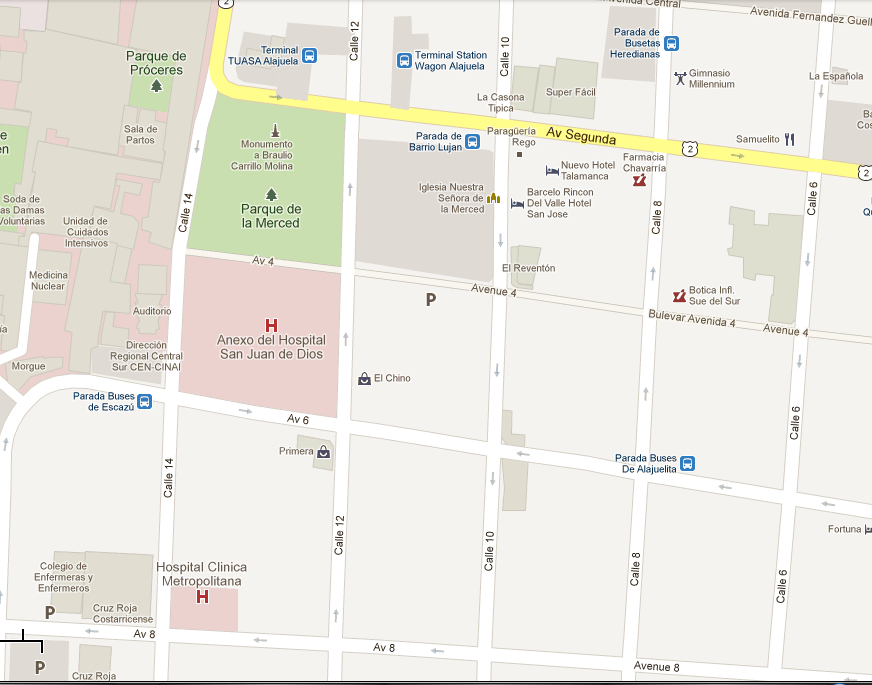
\includegraphics[scale=0.37]{images/trafico1.png}
\caption{Diagrama de Calles, San Jos\'e Costa Rica (Google Maps)}
\label{fig:traficoSJ}
\end{figure}

		Basado en dicha imagen, se plantea el problema de cambio de las luces de los
	sem\'{a}foros tomando como referencia la \textbf{avenida:} 2, 4, 6 y 8,  y las
	\textbf{calles:}
	12, 10, 8 y 6. Para este caso la avenida segunda (Juan Rafael Mora Porras) se ve afectada fuertemente por los veh\'{i}culos automotores que quedan en medio de las intersecciones, si bien es ilegal, este se mantiene como un problema m\'{a}s cultural.
			
	Dependiendo de las condiciones en ese momento, ya sea un alto n\'{u}mero de
	veh\'{i}culos automotores en la cercan\'{i}a o la presencia de una fuerte lluvia que
	dificulte la conducci\'{o}n, es probable que se genere un efecto en cadena el cual
	culminar\'{a} afectando, con igual o mayor rapidez, otras \'{a}reas.

	Es aqu\'{i} donde la primera parte de este trabajo (la simulaci\'{o}n) se pone en funcionamiento. Para este caso la simulaci\'{o}n s\'{o}lo comprender\'{a} escenarios normales dentro de la zona, si ningun evento o factor que altere la presencia o el flujo de veh\'{i}culos dentro de la misma. Otro aspecto importante a considerar es que el periodo a evaluarse corresponde a la franja horaria de las 4pm a las 6pm, dado que seg\'{u}n estimaciones realizadas en el MOPT, presenta una tendencia de flujo m\'{a}s constante en comparaci\'{o}n con las horas de la ma\~{n}ana donde se obtienen picos pronunciados en menor tiempo, correspondientes al traslado de personas a su lugar de trabajo.
	
	Siguiendo estas consideraciones, la simulaci\'{o}n a implementar tomar\'{a} en cuenta la llegada de veh\'{i}culos a la zona por medio de las calles o avenidas que conducen hacia la zona, es decir, calles cuya direcci\'{o}n o sentido llevan a los conductores hacia el \'{a}rea mencionada. De igual forma, se debe garantizar la circulaci\'{o}n de los veh\'{i}culos en las calles. Por lo anterior, en caso de presentarse una obstrucci\'{o}n en alg\'{u}n carril los carros deben ser capaces de realizar el cambio a un carril adyacente, teniendo en cuenta que cada calle tiene al menos dos carriles disponibles, salvo los casos como la avenida segunda la cual cuenta hasta con cinco, o las calles y avenidas que poseean zonas de carga y descarga que este puede reducirse a s\'{o}lo uno, no obstante este caso s\'{o}lo se presenta una vez dentro de la zona.

	Finalmente, los veh\'{i}culos han de circular dentro del \'{a}rea y en cada intersecci\'{o}n tomar\'{a}n una decisi\'{o}n si continuan en l\'{i}nea recta o si dan vuelta en la calle, \'{e}sto basado en el destino que cada automotor tenga. Para todos los casos a saber: cambios de carril, llegada de veh\'{i}culos y tendencias de flujos de los mismo, se han de emplear distribuciones probabil\'{i}sticas que permitan determinar cada uno de estos.
	
	Por otro lado y como etapa posterior, se ha pensado en la incorporaci\'{o}n a la simulaci\'{o}n de diferentes factores que alteren el flujo normal del tr\'{a}fico, \'{e}stos pueden darse de diferentes formas ya sea generando obstrucciones u obligando a reducciones de velocidades, sin importar el caso todos repercuten en cierta forma las calles por medio de los congestionamientos que generan.
	
\subsection{Factores a Considerarse}
Los factores se obtienen con base en los eventos y condiciones que tienden a presentarse en la mayor\'{i}a de zonas del pa\'{i}s.

Cada factor consta de dos a tres niveles a ser tomados en cuenta, dichos niveles implica un diferente nivel de dificultad para el avance normal de los otros veh\'{i}culos dentro de la zona. Los factores se explican a continuaci\'{o}n.

\subsubsection{Accidentes de Tr\'{a}nsito}
Para la selecci\'{o}n de estos se tom\'{o} como base el mapa de distribuci\'{o}n espacial de accidentes para la zona obtenido del “Estudio de la distribuci\'{o}n espacial de accidentes de tr\'{a}nsito con v\'{i}ctimas en el cant\'{o}n de San Jos\'{e}” el cual fue proporcionado por el Consejo de Seguridad Vial. Para estos casos se utilizaron calles o avenidas de la zona que, de acuerdo con el estudio, presentan una mayor concentraci\'{o}n de accidentes.

\subsubsection{Zonas de Parqueos}
La idea de este  factor corresponde a un hecho caracter\'{i}stico como lo son paradas de autobuses, zonas de descarga y terminales en las calles. Si se analiza considerando que las calles posean un m\'{a}ximo de 2 carriles se pueden notar los siguientes comportamientos: si se poseen terminales de buses, se habla de un carril pr\'{a}cticamente dedicado a estas, mientras que para el otro caso se poseen bloqueos temporales de un carril en ciertos puntos por un tiempo determinado como resultado de que los buses realicen paradas para subir o bajar pasajeros. 

	Cabe mencionar que para este caso s\'{o}lo se considerar\'{a}n casos de paradas permanentes, por el hecho de que realizar evaluaciones de otros resulta bastante dif\'icil debido al grado de variaci\'on que se presenta, tal es el caso de el parqueo temporal de veh\'iculos el cual depender\'a de cada persona, seg\'un las habilidades y experiencia con las que cuenten para tardar m\'as o menos tiempo en estacionar un veh\'iculo.

\subsubsection{Eventos Meteorol\'{o}gicos}
Este factor var\'{i}a mucho pero igual se encuentra presente dentro de los factores que afectan y resulta necesario ser considerado. Para este caso, la presencia de lluvia en San Jos\'{e} ser\'{a} la principal circunstancia a evaluar tomando como punto de partida el hecho de que al presentarse, los conductores tienden a reducir la velocidad con el fin de evitar accidentes por las dificultades para manejar que se presentan con la calle mojada o la poca visibilidad en caso de una lluvia fuerte.

\subsubsection{Condiciones de los sem\'aforos}
Uno de los principales factores que deben de considerarse es el estado de los sem\'aforos, indicando qu\'e calles y avenidas est\'an avanzando y cu\'ales est\'an detenidas. Este factor debe de poder ser controlado de manera din\'amica, para poder buscar mejoras posteriores, al ser el \'unico sobre el cual se tiene control externo, a diferencia de los mencionados anteriormente.


\section{Distribuciones de probabilidad a Emplear}
Al entrevistar a expertos del Consejo Nacional de Vialidad (CONAVI), Consejo de Seguridad Vial (COSEVI) y del MOPT, se lograron obtener registros del comportamiento muestral de los veh\'iculos en los \'ultimos a\~nos en nuestra capital. 

\subsection{Entrada de veh\'iculos}
La hora (con segundos) de llegada de veh\'iculos se obtiene a partir de una distribuci\'on de Poisson, cuya media var\'ia de acuerdo con las horas del d\'ia. Donde la media de menor valor corresponde con el per\'iodo comprendido entre las cuatro de la tarde y las siete de la noche, con una media de 5. Esto quiere decir que en promedio, entra un autom\'ovil cada cinco segundos por cada una de las posibles entradas. Es interesante como una muestra similar se puede apreciar entre las siete y ocho de la ma\~nana, sin embargo, en este evento, los autos transitan con mayor premura, debido a que muchos van a hacer su ingreso a su lugar de trabajo lo que agiliza significativamente el tr\'ansito.

\subsection{Velocidad de los veh\'iculos}
Los veh\'iculos mantienen una velocidad normal con media de 44 km/h y una desviaci\'on est\'andar de 3 km/h. 

\subsection{Ceder el paso}
En caso de alg\'un bloqueo u obstrucci\'on en la carretera, tal como pueden ser autobuses estacionados, accidentes de tr\'ansito o cualquier otro tipo de evento, es importante encontrar cu\'al es la cantidad de veh\'iculos que van a pasar antes de que uno le ceda el paso a otro veh\'iculo que ve impedido su avance por el evento obstaculizador. Este n\'umero de veh\'iculos que pasan sin ceder el campo est\'a dado por una distribuci\'on geom\'etrica y la probabilidad P, var\'ia muy poco a pesar del n\'umero de veh\'iculos o de la hora. Siendo la menor $0.1$ y la mayor $0.2$ 

\subsection{Giro en las intersecciones}
En cada intersecci\'on la probabilidad de giro de un veh\'iculo particular en una intersecci\'on cualquiera var\'ia muy poco, dado que los usuarios normalmente utilizan la misma ruta siempre. Una vez m\'as, para agilizar la ejecuci\'on de la simulaci\'on, se utiliz\'o una distribuci\'on geom\'etrica para indicar el n\'umero de veh\'iculos que iban a continuar directamente sobre una intersecci\'on antes de que uno gire. Naturalmente esta probabilidad se ve afectada por eventos como obras en la v\'ia, marchas de protesta o accidentes de tr\'ansito, lo que debe de ser considerado por el sistema.


\section{Resultados}

Como parte de los resultados que se pueden obtener del simulador en las siguientes secciones se mencionan en detalles los m\'as importantes.

\subsection{Informaci\'on de los carros}

Para cada uno de los carros, se almacenan diferentes datos relativos a su permanencia dentro de la zona de evaluaci\'on, a saber: Tiempo de espera total, demora total, posici\'on dentro de la l\'inea actual. Para el caso del tiempo de espera, este corresponde a un valor acumulado que se incrementa en cada iteraci\'on de la simulaci\'on y cuyo valor final corresponde a la suma de los tiempos de espera acumulados por cada calle o avenida que el veh\'iculo tuvo que circular hasta llegar a su destino fuera del area. 

	Por otro lado, la demora total corresponde a los tiempos acumulados para los carros, que se generen por eventos que causen atrasos a estos como el caso de obstrucciones en las v\'ia o que las calles han llegado al m\'aximo de su capacidad y por lo tanto tienen que esperar fuera de estas para poder ingresar y continuar con la ruta. Finalmente se cuenta con la posici\'on de los automotores en cada calle, para este caso debe tenerse en cuenta que la posici\'on es \'unica para cada calle y al momento de que se pase a una nueva la misma ser\'a reiniciada al valor m\'aximo posible dependiendo de la capacidad de la calle.

	Como \'ultimo dato y a modo de referencia, al iniciar su ingreso al \'area, cada veh\'iculo contar\'a con una decisi\'on que tomar para determinar la ruta a seguir, esto basado en las distribuciones mencionadas anteriormente. A modo de evaluaci\'on posterior, se contar\'a con un registro de las avenidas y calles recorridas de forma que pueda determinarse si la ruta tomada se vio afectada por alg\'un evento o si esta puede corresponder a una ruta adecuada considerando el tiempo invertido por veh\'iculo y el destino de \'este. 

\subsection{Informaci\'on de los sem\'aforos}

A modo de registro, y como una forma de control y an\'alisis de las decisiones tomas, cada sem\'aforo contar\'a con un archivo de log o registro el cual permita en etapas posteriores, hacer revisiones de los movimientos realizados por esto. Dicha informaci\'on se tiene en fin de poder hacer revisiones manuales en casos de buscar mejoras en comportamientos del sem\'aforo cuando sea empleado en las etapas posteriores del proyecto.  

\section{Trabajo Futuro}

Resulta destacable hay algunos datos que se obtienen que no pueden verificarse su exactitud debido a que a la fecha, ninguna entidad gubernamental o privada posee datos sobre ciertos tipos de comportamientos extraños en los ciudadanos, como el caso de un choque leve donde se arreglan por su parte y no se hace el reporte a la oficina de tr\'ansito. Por lo que el modelo puede ser inexacto ante eventualidades como esta, de modo que si se instalan sensores que indiquen comportamientos extraños, entonces se puede retroalimentar al simulador.

Posterior a la realizaci\'{o}n del modelo de simulaci\'{o}n, es importante encontrar un mecanismo que agilice el control del tr\'ansito. En el proceso pretende lograr un modelo de red neuronal artificial que pueda ser implementada dentro de este red de sem\'{a}foros y el cual permita que cada sem\'{a}foro se comunique con otros (hermanos) localizados dentro de un rango de \'{a}rea considerable de forma que cada uno pueda tener una idea lo que ocurre en su entorno y no \'{u}nicamente la informaci\'{o}n que puede ser recolectada por medio de los sensores en la intersecci\'{o}n administrada por cada sem\'{a}foro.

\subsection{Uso de Redes Neuronales}
La idea de usar redes neuronales, se basa en el hecho de que actualmente los sem\'{a}foros no son realmente inteligentes a como fueron promocionados en un principio. Dado que hacen uso de tiempos fijos, preprogramados, las tendencias cambiantes del flujo puede no siempre lograr satisfacer de forma adecuada la demanda real. Si bien los flujos de veh\'{i}culos siguien ciertas tendencias, de alzas o bajas, esto suele ser de constante cambio y en algunos momentos puede requerirse de ajustes inmediatos seg\'{u}n datos que se hayan analizado.

Dato que las redes neuronales se entrenan para aprender a generalizar resultados, lo que se busca es lograr que esta luego de un entrenamiento pueda conocer los momentos en los que de se debe aumentar o disminuir el tiempo de la luz verde, basado en su conocimiento actual tanto de la informaci\'{o}n recopilada por sensores como el insumo brindado por otros sem\'{a}foros cercanos.

\subsection{Algoritmos alternativos}
Otro algoritmos posible para contrastar el rendimiento pueden ser:
\begin{enumerate}
\item Cadenas de Markov
\item Redes Bayesianas
\item Modelo MM1 de colas
\item Modelo MMc de colas
\item Modelo MG1 de colas
\item Redes Causales
\end{enumerate}
		
\section{Conclusi\'on}
Como principal conclusi\'on se tiene que se ha logrado montar un modelo exitoso que permite la simulaci\'on de San Jos\'e con sus particularidades. Tambi\'en se cuenta con una herramienta de evaluaci\'on para las posibles pol\'iticas viales que se puedan proponer en nuestro ambiente. 

Las particularidades de la sociedad costarricense aunado a un espacio vial reducido que por lo general se encuentra a\'un m\'as reducido por diversas razones, se ve reflejado de manera muy similar a la realidad en el sistema de simulaci\'on

Las variables obtenidas de los expertos, permitieron que el modelo se completara y se pudiera ajustar a los detalles que satisfacen las condiciones precisas y los resultados obtenidos se pueden ajustar para diferentes horarios del d\'ia.





% if have a single appendix:
%\appendix[Proof of the Zonklar Equations]
% or
%\appendix  % for no appendix heading
% do not use \section anymore after \appendix, only \section*
% is possibly needed

% use appendices with more than one appendix
% then use \section to start each appendix
% you must declare a \section before using any
% \subsection or using \label (\appendices by itself
% starts a section numbered zero.)
%


\appendices
\section{Erlang como lenguaje de desarrollo}
Las caracter\'isticas de Erlang que permiten que la creaci\'on de hilos de manera sencilla, hizo que se pudieran modelar cada uno de los componentes del simulador como un hilo individual y se crearon funciones especializadas en coordinar la sincronizaci\'on de los diversos hilos, de modo que cada uno de ellos fuera individual, haciendo m\'as realista la simulaci\'on.

% use section* for acknowledgement
\ifCLASSOPTIONcompsoc
  % The Computer Society usually uses the plural form
  \section*{Agradecimiento}
\else
  % regular IEEE prefers the singular form
  \section*{Agradecimientos}
\fi


Los autores les gustar\'ia agradecer muy profundamente al COSEVI, CONAVI y MOPT por su invaluable apoyo, la atenci\'on brindada y los datos mostrados, sin los cuales este paper no habr\'ia sido posible. En particular a quienes han dedicado su tiempo en la revisi\'on de este material para su validaci\'on.%MAG ac\'a van los nombres y puestos de las personas que te han ayudado...


% Can use something like this to put references on a page
% by themselves when using endfloat and the captionsoff option.
\ifCLASSOPTIONcaptionsoff
  \newpage
\fi



% trigger a \newpage just before the given reference
% number - used to balance the columns on the last page
% adjust value as needed - may need to be readjusted if
% the document is modified later
%\IEEEtriggeratref{8}
% The "triggered" command can be changed if desired:
%\IEEEtriggercmd{\enlargethispage{-5in}}

% references section

% can use a bibliography generated by BibTeX as a .bbl file
% BibTeX documentation can be easily obtained at:
% http://www.ctan.org/tex-archive/biblio/bibtex/contrib/doc/
% The IEEEtran BibTeX style support page is at:
% http://www.michaelshell.org/tex/ieeetran/bibtex/
%\bibliographystyle{IEEEtran}
% argument is your BibTeX string definitions and bibliography database(s)
%\bibliography{IEEEabrv,../bib/paper}
%
% <OR> manually copy in the resultant .bbl file
% set second argument of \begin to the number of references
% (used to reserve space for the reference number labels box)

%\bibliographystyle{IEEEtran}
%\bibliography{IEEEabrv, IEEEreferences}
\begin{thebibliography}{1}

\bibitem{HPerros}
H.Perros, \emph{Computer Simulation Techniques:
The definitive introduction!}, 2009. Computer Science Department. NC State University. Raleigh, NC. http://www4.ncsu.edu/~hp/simulation.pdf

\bibitem{SWeppner}
S.Weppner, \emph{Computational methods with depth and Flair}, September/October 2008. IEEE CS and the AIP. http://www2.computer.org/cms/Computer.org/
ComputingNow/bookreviews/archive/CiSE\%204.pdf 

\bibitem{NDaneshjo}
N.Daneshjo, \emph{Computer Modeling and Simulation},2011. Sinaia, Romania.
http://www.ipcsit.com/vol8/12-S3.3.pdf

\bibitem{Villegas2012}
J. Villegas and L.Herrera, \emph{260.000 autos y 19.000 buses atascan San Jos\'{e} cada d\'{\i}a}, 2012, La Naci\'{o}n. San Jos\'{e}, Costa Rica. http://www.nacion.com/2012-03-17/ElPais/260-000-autos-y-19-000-buses-atascan-san-jose-cada-dia.aspx

\bibitem{Loaiza2007}
 V.Loaiza, \emph{Capital estrena sem\'{a}foros inteligentes en 180 intersecciones}, 2007. La Naci\'{o}n. San Jos\'{e}, Costa Rica. 
http://wvw.nacion.com/ln\_ee/2007/noviembre/28
/pais1332560.html

\bibitem{Mata2009}
A.Mata, \emph{Acceso libre a San Jos\'{e} provoca colapso vial}, 2009. La Naci\'{o}n. San Jos\'{e}, Costa Rica. 
http://wvw.nacion.com/ln\_ee/2009/junio/16/pais1997637.html

\end{thebibliography}




% An example of a floating figure using the graphicx package.
% Note that \label must occur AFTER (or within) \caption.
% For figures, \caption should occur after the \includegraphics.
% Note that IEEEtran v1.7 and later has special internal code that
% is designed to preserve the operation of \label within \caption
% even when the captionsoff option is in effect. However, because
% of issues like this, it may be the safest practice to put all your
% \label just after \caption rather than within \caption{}.
%
% Reminder: the "draftcls" or "draftclsnofoot", not "draft", class
% option should be used if it is desired that the figures are to be
% displayed while in draft mode.
%
%\begin{figure}[!t]
%\centering
%\includegraphics[width=2.5in]{myfigure}
% where an .eps filename suffix will be assumed under latex, 
% and a .pdf suffix will be assumed for pdflatex; or what has been declared
% via \DeclareGraphicsExtensions.
%\caption{Simulation Results}
%\label{fig_sim}
%\end{figure}

% Note that IEEE typically puts floats only at the top, even when this
% results in a large percentage of a column being occupied by floats.


% An example of a double column floating figure using two subfigures.
% (The subfig.sty package must be loaded for this to work.)
% The subfigure \label commands are set within each subfloat command, the
% \label for the overall figure must come after \caption.
% \hfil must be used as a separator to get equal spacing.
% The subfigure.sty package works much the same way, except \subfigure is
% used instead of \subfloat.
%
%\begin{figure*}[!t]
%\centerline{\subfloat[Case I]\includegraphics[width=2.5in]{subfigcase1}%
%\label{fig_first_case}}
%\hfil
%\subfloat[Case II]{\includegraphics[width=2.5in]{subfigcase2}%
%\label{fig_second_case}}}
%\caption{Simulation results}
%\label{fig_sim}
%\end{figure*}
%
% Note that often IEEE papers with subfigures do not employ subfigure
% captions (using the optional argument to \subfloat), but instead will
% reference/describe all of them (a), (b), etc., within the main caption.


% An example of a floating table. Note that, for IEEE style tables, the 
% \caption command should come BEFORE the table. Table text will default to
% \footnotesize as IEEE normally uses this smaller font for tables.
% The \label must come after \caption as always.
%
%\begin{table}[!t]
%% increase table row spacing, adjust to taste
%\renewcommand{\arraystretch}{1.3}
% if using array.sty, it might be a good idea to tweak the value of
% \extrarowheight as needed to properly center the text within the cells
%\caption{An Example of a Table}
%\label{table_example}
%\centering
%% Some packages, such as MDW tools, offer better commands for making tables
%% than the plain LaTeX2e tabular which is used here.
%\begin{tabular}{|c||c|}
%\hline
%One & Two\\
%\hline
%Three & Four\\
%\hline
%\end{tabular}
%\end{table}


% Note that IEEE does not put floats in the very first column - or typically
% anywhere on the first page for that matter. Also, in-text middle ("here")
% positioning is not used. Most IEEE journals/conferences use top floats
% exclusively. Note that, LaTeX2e, unlike IEEE journals/conferences, places
% footnotes above bottom floats. This can be corrected via the \fnbelowfloat
% command of the stfloats package.








% trigger a \newpage just before the given reference
% number - used to balance the columns on the last page
% adjust value as needed - may need to be readjusted if
% the document is modified later
%\IEEEtriggeratref{8}
% The "triggered" command can be changed if desired:
%\IEEEtriggercmd{\enlargethispage{-5in}}

% references section

% can use a bibliography generated by BibTeX as a .bbl file
% BibTeX documentation can be easily obtained at:
% http://www.ctan.org/tex-archive/biblio/bibtex/contrib/doc/
% The IEEEtran BibTeX style support page is at:
% http://www.michaelshell.org/tex/ieeetran/bibtex/
%\bibliographystyle{IEEEtran}
% argument is your BibTeX string definitions and bibliography database(s)
%\bibliography{IEEEabrv,../bib/paper}
%
% <OR> manually copy in the resultant .bbl file
% set second argument of \begin to the number of references
% (used to reserve space for the reference number labels 




% that's all folks
\end{document}


